\def\duedate{\today}
\def\HWnum{5}
\documentclass[10pt,a4paper]{book}

% custom section formatting
\usepackage{titlesec}
\titleformat{\chapter}[display]
{\normalfont\Large\filcenter\sffamily}
{\titlerule[1pt]%
\vspace{1pt}%
\titlerule
\vspace{1pc}%
\LARGE\MakeUppercase{\chaptertitlename} \thechapter}
{1pc}
{\titlerule
\vspace{1pc}%
\Huge}

% appendix handling
\usepackage[toc,page]{appendix}
    
% encoding for file and font
\usepackage[utf8]{inputenc}
\usepackage[T1]{fontenc}

% math formatting/tools
\usepackage{amsmath}
\usepackage{amssymb}
\usepackage{mathtools}
\usepackage[arrowdel]{physics}

% unit formatting
\usepackage{siunitx}
\AtBeginDocument{\RenewCommandCopy\qty\SI}

% figure formatting/tools
\usepackage{graphicx}
\usepackage{float}
\usepackage{subcaption}
\usepackage{multirow}
\usepackage{import}
\usepackage{pdfpages}
\usepackage{transparent}
\usepackage{currfile}

\NewDocumentCommand\incfig{O{1} m}{
    \def\svgwidth{#1\textwidth}
    \import{./Figures/\currfiledir}{#2.pdf_tex}
}

\newcommand{\bef}{\begin{figure}[h!tb]\centering}
\newcommand{\eef}{\end{figure}}

\newcommand{\bet}{\begin{table}[h!tb]\centering}
\newcommand{\eet}{\end{table}}

% hyperlink references 
\usepackage{hyperref}
\hypersetup{
    colorlinks=true,
    linkcolor=blue,
    filecolor=magenta,
    urlcolor=cyan,
    pdftitle={Physics 1 Notes},
    pdfauthor={Richard Whitehill},
    pdfpagemode=FullScreen
}
\urlstyle{same}

\newcommand{\eref}[1]{Eq.~(\ref{eq:#1})}
\newcommand{\erefs}[2]{Eqs.~(\ref{eq:#1})--(\ref{eq:#2})}

\newcommand{\fref}[1]{Fig.~(\ref{fig:#1})}
\newcommand{\frefs}[2]{Fig.~(\ref{fig:#1})--(\ref{fig:#2})}

\newcommand{\aref}[1]{Appendix~(\ref{app:#1})}
\newcommand{\sref}[1]{Section~(\ref{sec:#1})}
\newcommand{\srefs}[2]{Sections~(\ref{sec:#1})-(\ref{sec:#2})}

\newcommand{\tref}[1]{Table~(\ref{tab:#1})}
\newcommand{\trefs}[2]{Table~(\ref{tab:#1})--(\ref{tab:#2})}

% tcolorbox formatting/definitions
\usepackage[most]{tcolorbox}
\usepackage{xcolor}
\usepackage{xifthen}
\usepackage{parskip}

\definecolor{peach}{rgb}{1.0,0.8,0.64}

\DeclareTColorBox[auto counter, number within=chapter]{defbox}{O{}}{
    enhanced,
    boxrule=0pt,
    frame hidden,
    borderline west={4pt}{0pt}{green!50!black},
    colback=green!5,
    before upper=\textbf{Definition \thetcbcounter \ifthenelse{\isempty{#1}}{}{: #1} \\ },
    sharp corners
}

\newcommand*{\eqbox}{\tcboxmath[
    enhanced,
    colback=black!10!white,
    colframe=black,
    sharp corners,
    size=fbox,
    boxsep=8pt,
    boxrule=1pt
]}

\newtcolorbox[auto counter, number within=chapter]{exbox}{
    parbox=false,
    breakable,
    enhanced,
    sharp corners,
    boxrule=1pt,
    colback=white,
    colframe=black,
    before upper= \textbf{Example \thetcbcounter:}\,,
    before lower= \textbf{Solution:}\,,
    segmentation hidden
}

\newtcolorbox{resbox}{
    enhanced,
    colback=black!10!white,
    colframe=black,
    boxrule=1pt,
    boxsep=0pt,
    top=2pt,
    ams nodisplayskip,
    sharp corners
}


\begin{document}

\prob{1}{

(a) Two halves of a long hollow conducting cylinder of inner radius $b$ are separated by small lengthwise gaps on each side, and are kept at different potentials $V_1$ and $V_2$.
Show that the potential inside is given by 
\begin{eqnarray}
    \Phi(s,\phi) = \frac{V_1 + V_2}{2} + \frac{V_1 - V_2}{\pi} \arctan(\frac{2 b s}{b^2 - s^2} \cos{\phi})
,\end{eqnarray}
where $\phi$ is measured from a plane perpendicular to the plane through the gap.

(b) Calculate the surface-charge density on each half of the cylinder.

}

\sol{

In polar coordinates with translational symmetry along the $z$ axis, Laplace's equation reads
\begin{eqnarray}
    \laplacian \Phi = \frac{1}{s} \pdv{s} \Big( s \pdv{\Phi}{s} \Big) + \frac{1}{s^2} \pdv[]{\Phi}{s}
.\end{eqnarray}
We can guess an ansatz for a particular solution as
\begin{eqnarray}
    \Phi(s,\phi) = R(s) T(\phi)
,\end{eqnarray}
which gives two separate second-order ordinary differential equations for the $s$ and $\phi$ dependence:
\begin{gather}
    s \dv{s}\Big( s \dv{R}{s} \Big) - \nu^2 R = 0 \\
    \dv[2]{T}{\phi} + \nu^2 T = 0
.\end{gather}
Note that we have written these equations choosing the sign of $\nu^2$ with the foresight that $T$ must be cyclic (i.e. $T(\phi + 2\pi) = T(\phi)$).
Thus, we can write the general solution
\begin{eqnarray}
    \Phi(s,\phi) = (a_0 + b_0 \ln{s})(A_0 + B_0 \phi) + \sum_{\nu > 0} (a_{\nu} s^{\nu} + b_{\nu} s^{-\nu}) (A_{\nu} \cos{\nu \phi} + B_{\nu} \sin{\nu \phi})
.\end{eqnarray}
Since we are interested in $\Phi$ in the region $s \leq b$, we must have $b_0 = b_{\nu} = 0$ such that $\Phi$ is finite.
Let us then write
\begin{eqnarray}
    \Phi(s,\phi) = A_0 + B_0 \phi + \sum_{\nu > 0} [A_{\nu} \cos{\nu \phi} + B_{\nu} \sin{\nu \phi} ] s^{\nu}
,\end{eqnarray}
where we have absorbed the constants $a_{\nu}$ into $A_{\nu}$ and $B_{\nu}$.
Note that since $\Phi(s,\phi + 2\pi) = \Phi(s,\phi)$, we must have $B_0 = 0$ and $\nu = n \in \naturals$\footnote{Equating $\Phi(s,\phi+2\pi)$ and $\Phi(s,\phi)$, we get the equations $2\pi B_0 = 0$, $\cos(2\pi\nu) + \sin(2\pi\nu) = 1$, and $\cos(2\pi\nu) - \sin(2\pi\nu) = 1$, which reduces to $\sin(2\pi\nu) = 0$ and $\cos(2\pi\nu) = 1$ which are only satisfied if $2\pi\nu = 2 \pi n$ or $\nu = n$.}, which leaves us with
\begin{eqnarray}
    \Phi(s,\phi) = A_0 + \sum_{n=1}^{\infty} [A_{n} \cos(n\phi) + B_{n} \sin(n\phi)] s^{n}
.\end{eqnarray}
We can solve for the $A_{n}$ and $B_{n}$ using the orthogonality relations (for $n > 0$)
\begin{align}
    \int_{-\pi}^{\pi} \sin(mx)\sin(nx) \dd{x} &= \pi \delta_{nm} \\
    \int_{-\pi}^{\pi} \sin(mx)\cos(nx) \dd{x} &= 0 \\
    \int_{-\pi}^{\pi} \cos(mx)\cos(nx) \dd{x} &= \pi \delta_{nm}
,\end{align}
where $\delta_{nm}$ is the kronecker-delta symbol.
Hence, letting (note that I first solved the problem with the angle measured from the plane splitting the half-cylinders, so I will correct that mistake by taking $\phi \rightarrow \phi + 2\pi$ in the final results).
\begin{eqnarray}
   \Phi(b,\phi) = \begin{cases}
       V_2 & -\pi < \phi < 0 \\
       V_1 & 0 < \phi < \pi
   .\end{cases}
\end{eqnarray}

\begin{align}
    A_0 &= \frac{1}{2\pi} \int_{-\pi}^{\pi} \Phi(b,\phi) \dd{\phi} = \frac{V_1 + V_2}{2} \\
    A_{n>0} &= \frac{1}{\pi b^{n}} \int_{-\pi}^{\pi} \Phi(b,\phi) \cos(n\phi) \dd{\phi} = 0 \\
    B_{n>0} &= \frac{1}{\pi b^{n}} \int_{-\pi}^{\pi} \Phi(b,\phi) \sin(n\phi) \dd{\phi} = \frac{1}{\pi b^{n}} \frac{V_1 - V_2}{n} [1 - (-1)^{n}]
.\end{align}
Putting this into the expression for $\Phi$, we arrive at
\begin{eqnarray}
    \Phi(s,\phi) = \frac{V_1 + V_2}{2} + \frac{V_1 - V_2}{\pi} \Bigg[ 2 \sum_{n=0}^{\infty} \frac{\sin[(2n+1)\phi]}{n} \Big( \frac{s}{b} \Big)^{2n+1} \Bigg]
.\end{eqnarray}

Finally, we only have to find the value of the series in the second term.
We do so by writing
\begin{eqnarray}
    S = 2\sum_{n=0}^{\infty} \frac{\sin[(2n+1) \phi]}{n} \Big( \frac{s}{b} \Big)^{2n+1} = \Im{ 2\sum_{n=0}^{\infty} \frac{1}{n} \Big( \frac{s}{b} e^{i\phi} \Big)^{2n+1} } \\
.\end{eqnarray}
Recall that
\begin{align}
    \ln(1 + x) &= \sum_{n=0}^{\infty} \frac{(-1)^{n+1}}{n} x^{n} = -\sum_{n=0}^{\infty} \frac{x^{2n}}{2n} + \sum_{n=0}^{\infty} \frac{x^{2n+1}}{2n+1} \\
    \ln(1 - x) &= \sum_{n=0}^{\infty} \frac{(-1)^{n+1}}{n} (-1)^{n} x^{n} = -\sum_{n=0}^{\infty} \frac{x^{2n}}{2n} - \sum_{n=0}^{\infty} \frac{x^{2n+1}}{2n+1} \\
    &\Rightarrow \ln(1 + x) - \ln(1 - x) =\ln( \frac{1 + x}{1-x} ) = 2 \sum_{n=0}^{\infty} \frac{x^{2n+1}}{2n + 1}
,\end{align}
and therefore, we can write\footnote{Notice that $(b+s e^{i\phi})(b - s e^{-i\phi}) = (b^2 - s^2) + 2i b s \sin{\phi}$.}
\begin{eqnarray}
    S = \Im{ \ln( \frac{1 + (s/b)e^{i\phi}}{1 - (s/b)e^{i\phi}} ) } = \arctan\Bigg[ \frac{2 s b \sin{\phi}}{b^2 - s^2} \Bigg]
.\end{eqnarray}

We then arrive at the result
\begin{eqnarray}
    \Phi(s,\phi) = \frac{V_1 + V_2}{2} + \frac{V_1 - V_2}{\pi} \arctan( \frac{2bs \sin{\phi}}{b^2 - s^2} )
,\end{eqnarray}
and carrying out the transformation $\phi \rightarrow \phi + \pi/2$ as promised, the final result is
\begin{eqnarray}
    \eqbox{ \Phi(s,\phi) = \frac{V_1 + V_2}{2} + \frac{V_1 - V_2}{\pi} \arctan(\frac{2bs \cos{\phi}}{b^2 - s^2}) }
\end{eqnarray}
since $\sin(\phi + \pi/2) = \sin{\phi} \cos{\pi/2} + \sin{\pi/2}\cos{\phi} = \cos{\phi}$. 

(b) The surface charge density on each half of the sphere is given by
\begin{eqnarray}
\eqbox{
\begin{aligned}
    \sigma &= \epsilon_0 \pdv{\Phi}{s} \Big|_{s = b} = \epsilon_0 \frac{V_1 - V_2}{\pi} \frac{(b^2 - s^2)^2}{(b^2 - s^2)^2 + 4 b^2 s^2 \cos^2{\phi}} \frac{2b(b^2 + s^2)}{(b^2 - s^2)^2} \cos{\phi} \Big|_{s = b} \\
    &= \frac{\epsilon_0 (V_1 - V_2)}{\pi b \cos{\phi}}
.\end{aligned}
    }
\end{eqnarray}
Observe that if $\phi \in [-\pi/2,\pi/2]$ that $\sigma \sim V_1 - V_2$, while on $[\pi/2,3\pi/2]$ $\sigma \sim V_2 - V_1$, meaning that points on the cylinder reflected about the plane splitting the cylinder have surface charge densities of opposite sign but the same magnitude.
}


\prob{2}{

    A variant of the preceding two-dimensional problem is a long hollow conducting cylinder of radius $b$ that is divided into equal quarters, alternate segments being held at potential $+V$ and $-V$. \\[1pt]

(a) Solve by means of the series solution [See Eq. (2.71) in \textit{Jackson} and Eq. (13.5.9) in Lecture 10] and show that the potential inside the cylinder is
\begin{eqnarray}
    \Phi(s,\phi) = \frac{4V}{\pi} \sum_{n=0}^{\infty} \Big( \frac{s}{b} \Big)^{4n+2} \frac{\sin[(4n+2)\phi]}{2n+1}
.\end{eqnarray}

(b) Sum the series and show that
\begin{eqnarray}
    \Phi(s,\phi) = \frac{2V}{\pi} \arctan(\frac{2 s^2 b^2 \sin{2\phi}}{b^{4} - s^{4}})
.\end{eqnarray}

(c) Sketch the field lines and equipotentials.

}

\sol{

(a) We wrote down the generic solution for a setup such as this
\begin{eqnarray}
    \Phi(s,\phi) = A_0 + \sum_{n=1}^{\infty} [ A_{n}\cos(n\phi) + B_{n}\sin(n\phi) ] \Big( \frac{s}{b} \Big)^{n}
.\end{eqnarray}
Note that we have redefined our constants, anticipating that these factors will show up when we use the orthogonality relations: $A_{n} \rightarrow A_{n}/b^{n}$ and $B_{n} \rightarrow B_{n}/b^{n}$.
The constants are determined in the same way as in problem (1):
\begin{align}
    A_{0} &= \frac{1}{2\pi} \int_{-\pi}^{\pi} \Phi(b,\phi) \dd{\phi} = 0 \\
    A_{n > 0} &= \frac{1}{\pi} \int_{-\pi}^{\pi} \Phi(b,\phi) \cos(n\phi) \dd{\phi} = 0 \\
    B_{n > 0} &= \frac{1}{\pi} \int_{-\pi}^{\pi} \Phi(b,\phi) \sin(n\phi) \dd{\phi} = \frac{V}{\pi n} [ 1 - (-1)^{n} - 2\cos(\pi n /2) ]
,\end{align}
defining 
\begin{eqnarray}
    \Phi(b,\phi) = \begin{cases}
        +V & \phi \in (0,\pi/2) \cup (-\pi,-\pi/2) \\
        -V & \phi \in (\pi/2,\pi) \cup (-\pi/2,0) \\
    \end{cases}
.\end{eqnarray}
Note that the coefficients $B_{n}$ require a little more care this time.
We will write $n = 4k + r$, where $k \in \integers$ and $r \in \{ 0,1,2,3 \} $, which gives
\begin{eqnarray}
    B_{n} = \frac{2V}{\pi n} [1 + (-1)^{r} - 2 \cos(r \pi / 2)] = \frac{2V}{\pi n} \begin{cases}
        0 & r = 0 \\
        0 & r = 1 \\
        4 & r = 2 \\
        0 & r = 3
    \end{cases}
.\end{eqnarray}
Therefore, the series becomes
\begin{eqnarray}
    \eqbox{ \Phi(s,\phi) = \frac{4 V}{\pi} \sum_{n=0}^{\infty} \frac{\sin[(4n + 2) \phi]}{2n+1} \Big( \frac{s}{b} \Big)^{4n + 2} }
.\end{eqnarray}

(b) We can use the result of problem (1), taking $x \rightarrow x^2$, which gives
\begin{eqnarray}
    \ln(\frac{1 + x^2}{1 - x^2}) = 2 \sum_{n=0}^{\infty} \frac{x^{4n +2}}{2n+1}
\end{eqnarray}
and
\begin{eqnarray}
    2 \sum_{n=0}^{\infty} \frac{\sin[(4n+2)\phi]}{2n + 1} \Big( \frac{s}{b} \Big)^{4n+2} = \Im{ \ln(\frac{b^2 + s^2e^{2i\phi}}{b^2 - s^2 e^{2i\phi}}) } = \arctan( \frac{2b^2 s^2 \sin{2\phi}}{b^{4} - s^{4}} )
.\end{eqnarray}

Thus, we arrive at
\begin{eqnarray}
    \eqbox{ \Phi(s,\phi) = \frac{2 V}{\pi} \arctan( \frac{2b^2s^2 \sin{2\phi}}{b^{4} - s^{4}} ) }
.\end{eqnarray}

(c) If we write $s = b\xi$ and $x = \cos{\phi}$, $y = \sin{\phi}$, then the equipotential lines are given by
\begin{eqnarray}
    \label{eq:lcurves}
    \frac{4 x y (x^2 + y^2)}{1 - (x^2 + y^2)^2} = \tan(\frac{\pi}{2} \frac{\Phi}{V})
.\end{eqnarray}
Notice that $|\Phi| \leq V$ since $|\arctan{x}| \leq \pi/2$.
A plot of selected level curves is shown in \fref{prob2c-1}.

\begin{figure}[h!]
    \centering
    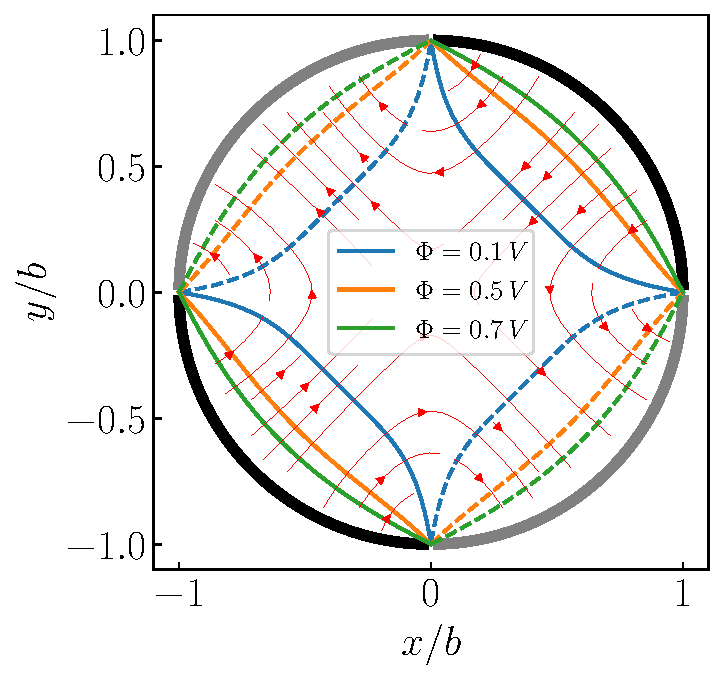
\includegraphics[width=0.5\textwidth]{prob2c-1.pdf}
    \caption{Plot of level curves satisfying \eref{lcurves} for a selection of $\Phi/V$, where the black and gray lines represent the portions of the cylinder held at potentials $\pm V$, respectively. Note that the solid lines are for $\Phi > 0$, while the dashed lines are the corresponding curves with $\Phi < 0$. The electric field lines are also imposed on the plot. Observe that the field lines are always perpendicular to the equipotential lines, and furthermore, they point from the positive}
    \label{fig:prob2c-1}
\end{figure}

}


\prob{3}{

A hollow cube has conducting walls defined by six planes $x = 0$, $y = 0$, $z = 0$ and $x = a$, $y=a$, $z = a$.
The walls $z = 0$ and $z = a$ are held at a constant potential $V$.
The other four sides are at zero potential. \\[1pt]

(a) Find the potential $\Phi(x,y,z)$ at any point inside the cube.

(b) Evaluate the potential at the center of the cube numerically, accurate to three significant figures.
How many terms in the series is it necessary to keep in order to attain this accuracy?
Compare your numerical result with the average value of the potential on the walls.

(c) Find the surface-charge density on the surface $z = a$.

}

\sol{

We proceed by a separable solution ansatz
\begin{eqnarray}
   \Phi(x,y,z) = X(x) Y(y) Z(Z)
,\end{eqnarray}
which gives
\begin{eqnarray}
    \frac{1}{X} \dv[2]{X}{x} + \frac{1}{Y}\dv[2]{Y}{y} + \frac{1}{Z}\dv[2]{Z}{z} = 0
.\end{eqnarray}
Each term must be constant given that they are each functions of separate independent variables.
Imposing boundary conditions for $x$ and $y$, we have
\begin{align}
    X_{n}(x) &= \sin(\frac{n \pi x}{a}) \\
    Y_{m}(y) &= \sin(\frac{m \pi x}{a})
.\end{align}
Immediately, we have
\begin{eqnarray}
    \dv[2]{Z}{z} = \frac{\pi^2 (n^2 + m^2)}{a^2} Z = \gamma_{nm}^2 Z
.\end{eqnarray}
Observe that we can solve the boundary value problem by writing $\Phi = \Phi_1 + \Phi_2$, where $\Phi_1(x,y,0) = 0$, $\Phi_1(x,y,a) = V$, $\Phi_2(x,y,0) = V$, and $\Phi_2(x,y,a) = 0$.
For the first solution we have
\begin{eqnarray}
   \Phi_1 = \sum_{n,m=1}^{\infty} A_{nm} \sin(\frac{n \pi x}{a}) \sin(\frac{m \pi x}{a}) \sinh(\gamma_{nm} z)
,\end{eqnarray}
while for the second solution we have
\begin{eqnarray}
    \Phi_2 = \sum_{n,m=1}^{\infty} B_{nm} \sin(\frac{n \pi x}{a}) \sin(\frac{m \pi x}{a}) \sinh[\gamma_{nm} (z - a)]
.\end{eqnarray}
We can use the orthogonality conditions to find
\begin{eqnarray}
    \begin{aligned}
        A_{nm} &= \Big( \frac{2}{a} \Big)^2 \frac{V}{\sinh(\gamma_{nm} a)} \int_{0}^{a} \dd{x} \sin(\frac{n \pi x}{a}) \int_{0}^{a} \dd{y} \sin(\frac{m \pi y}{a}) \\
               &= \frac{4}{a^2} \frac{V}{\sinh(\gamma_{nm}a)} \frac{a^2}{\pi^2 n m} [1 - (-1)^{n}][1 - (-1)^{m}] \\
               &= \begin{cases}
                   0 & n~{\rm or}~m \equiv 0 ~({\rm mod}~2) \\
                   \frac{16 V}{\pi^2 nm\sinh(\gamma_{nm} a)} & n,m \equiv 1 ~({\rm mod}~2)
               \end{cases}
    \end{aligned}
\end{eqnarray}
and
\begin{eqnarray}
    B_{nm} = -A_{nm}
.\end{eqnarray}
Hence,
\begin{eqnarray}
    \begin{aligned}
        \Phi(x,y,z) = \frac{16 V}{\pi^2} \sum_{n,m=0}^{\infty} \frac{1}{(2n+1)(2m+1)} &\sin(\frac{n \pi x}{a}) \sin(\frac{m \pi y}{a}) \\
                                                                                                             &\times \frac{\sinh(\gamma_{nm} z) - \sinh[\gamma_{nm} (z - a)]}{\sinh(\gamma_{nm} a)}
    \end{aligned}
,\end{eqnarray}
where we redefine $\gamma_{nm}^2 = \pi^2[(2n+1)^2 + (2m+1)^2]/a^2$.
Note that we can use the properties $\sinh{x} - \sinh{y} = 2\cosh[(x + y)/2]\sinh[(x - y)/2]$ and $\sinh{2x} = 2\sinh{x} \cosh{x}$ to write
\begin{eqnarray}
    \eqbox{ \Phi(x,y,z) = \frac{16 V}{\pi^2} \sum_{n,m=0}^{\infty} \frac{1}{(2n+1)(2m+1)}\sin(\frac{n \pi x}{a}) \sin(\frac{m \pi x}{a}) \frac{\cosh[\gamma_{nm} (z - a/2)]}{\cosh(\gamma_{nm} a/2)} }
.\end{eqnarray}

(b) We can make \tref{prob3} for the value of the sum after the first $N^2$ terms are computed.
\begin{table}[h!]
   \centering
   \begin{tabular}{c|c}
       \# of terms & $\Phi/V$ \\
       \hline
       1 & 0.347546 \\
       4 & 0.332958 \\
       9 & 0.333345 \\
       16 & 0.333333
   \end{tabular}
   \caption{Partial sums for $\Phi/V$ after the inclusion of $N^2$ terms.}
   \label{tab:prob3}
\end{table}
One can see that roughly after 9 terms (certainly after 16 terms), the partial sums are stable up to the third significant figure.
It appears actually that this result converges to about $1/3$, which interestingly is the average of the potential on the walls: $2V/6 = V/3$.

(c) The surface charge density on the plane $z = a$ is 
\begin{eqnarray}
    \eqbox{
    \begin{aligned}
        \sigma(x,y,a) &= \epsilon_0 \pdv{\Phi}{z}\Big|_{z=a} \\
                      &= \frac{16 \epsilon_0 V}{\pi^2} \sum_{n,m=1}^{\infty} \frac{\gamma_{nm}}{(2n+1)(2m+1)} \sin(\frac{n \pi x}{a}) \sin(\frac{m \pi x}{a}) \tanh(\gamma_{nm} a / 2) 
    .\end{aligned}
}
\end{eqnarray}


}


\prob{4}{

The two-dimensional region, $s \geq a$, $0 \leq \phi \leq \beta$ is bounded by conducting surfaces at $\phi = 0$, $s = a$, and $\phi = \beta$ held at zero potential, as indicated in the sketch.
At large $s$ the potential is determined by some configuration of charges and/or conductors at fixed potentials.

(a) Write down a solution for the potential $\Phi(s,\phi)$ that satisfies the boundary conditions for finite $s$.

(b) Keeping only the lowest nonvanishing terms, calculate the electric field components $E_{s}$ and $E_{\phi}$ and also the surface-charge densities $\sigma(s,0)$, $\sigma(s,\beta)$, and $\sigma(a,\phi)$ on the three boundary surfaces.

(c) Consider $\beta = \pi$ (a plane conductor with a half cylinder of radius $a$ on it).
Show that far from the half-cylinder the lowest order terms of part (b) give a uniform electric field normal to the plane.
Sketch the charge density on and in the neighborhood of the half-cylinder.
For fixed electric field strength far from the plane, show that the total charge on the half-cylinder (actually charge per unit length in the $z$ direction) is twice as large as would reside on a strip of width $2a$ in its absence.
Show that the extra portion is drawn from regions on the plane nearby, so that the total charge on a strip of width large compared to $a$ is the same whether the half-cylinder is there or not.

}

\sol{

(a) The generic series solution in this case is
\begin{eqnarray}
    \Phi(s,\phi) = (a_0 + b_0 \ln{s})(A_0 + B_0 \phi) + \sum_{\nu > 0} (a_{\nu}s^{\nu} + b_{\nu} s^{-\nu})(A_{\nu} \cos{\nu \phi} + B_{\nu} \sin{\nu \phi})
.\end{eqnarray}
We use the boundary condition at $\phi = 0$ first, which gives
\begin{eqnarray}
    (a_0 + b_0 \ln{s})A_0 + \sum_{\nu > 0} (a_{\nu} s^{\nu} + b_{\nu}s^{-\nu}) A_{\nu} = 0
.\end{eqnarray}
We can then immediately say $a_0A_0 = b_0A_0 = a_{\nu} A_{\nu} = b_{\nu} A_{\nu} = 0$, which leaves us with
\begin{eqnarray}
    \Phi = a_0 \phi + b_0 \phi \ln{s} + \sum_{\nu > 0} [a_{\nu} s^{\nu} +  b_{\nu} s^{-\nu}] \sin{\nu \phi}
,\end{eqnarray}
where we have absorbed $B_{\nu}$ into our definitions of $a_{\nu}$ and $b_{\nu}$.
Next, we have the condition at $\phi = \beta$, which gives
\begin{eqnarray}
    a_0 \beta + b_0 \beta \ln{s} + \sum_{\nu > 0} [ a_{\nu} s^{\nu} + b_{\nu} s^{-\nu} ] \sin{\nu \beta} = 0
,\end{eqnarray}
implying $a_0 = b_0 = 0$ and $\sin{\nu \beta} = 0$, which is equivalent to $\nu = n \pi/\beta$ for $n \in \naturals$.
The potential is then
\begin{eqnarray}
    \eqbox{ \Phi = \sum_{n=1}^{\infty} [a_{n} s^{n \pi / \beta} + b_{n} s^{-n \pi /\beta}] \sin(\frac{n \pi \phi}{\beta}) }
,\end{eqnarray}
and finally we use our condition at $s = a$, which gives
\begin{eqnarray}
    \sum_{n=1}^{\infty} [a_{n} a^{n \pi/\beta} + b_{n} a^{-n \pi/\beta}] \sin(\frac{n \pi \phi}{\beta}) = 0
.\end{eqnarray}
Thus, $b_{n} = -a^{2n\pi/\beta} a_{n}$.
Let us also redefine $a_{n} \rightarrow a_{n} a^{-n\pi/\beta}$, which gives
\begin{eqnarray}
    \eqbox{ \Phi(s,\phi) = \sum_{n=1}^{\infty} a_{n} \Big[ \Big( \frac{s}{a} \Big)^{n\pi/\beta} - \Big( \frac{a}{s} \Big)^{n\pi/\beta} \Big] \sin(\frac{n \pi \phi}{\beta}) }
.\end{eqnarray}

(b) With an expression for the potential, we can determine the electric field as
\begin{eqnarray}
    \va*{E} = -\pdv{\Phi}{s} \vu*{e}_{s} - \frac{1}{s}\pdv{\Phi}{\phi} \vu*{e}_{\phi}
,\end{eqnarray}
so
\begin{align}
    E_{s} &= - \pdv{\Phi}{s} = -\sum_{n=1}^{\infty} a_{n} \frac{n \pi}{a \beta} \Big[ \Big( \frac{s}{a} \Big)^{n\pi/\beta - 1} + \Big( \frac{a}{s} \Big)^{n\pi/\beta + 1} \Big] \sin(\frac{n \pi \phi}{\beta}) \nonumber \\
          &= \eqbox{ -a_1 \frac{\pi}{a \beta} \Big[ \Big( \frac{s}{a} \Big)^{\pi/\beta - 1} + \Big( \frac{a}{s} \Big)^{\pi/\beta + 1} \Big] \sin(\frac{\pi \phi}{\beta}) + \ldots } \\
    E_{\phi} &= -\frac{1}{s} \pdv{\Phi}{s} = -\sum_{n=1}^{\infty} a_{n} \frac{n\pi}{a\beta} \Big[ \Big( \frac{s}{a} \Big)^{n \pi/\beta - 1} - \Big( \frac{a}{s} \Big)^{n\pi/\beta + 1} \Big] \cos(\frac{n \pi \phi}{\beta}) \nonumber \\
             &= \eqbox{ -a_{1} \frac{\pi}{a \beta} \Big[ \Big( \frac{s}{a} \Big)^{\pi/\beta-1} - \Big( \frac{a}{s} \Big)^{\pi/\beta+1} \Big] \cos(\frac{\pi \phi}{\beta}) + \ldots }
.\end{align}
The surface charge densities along the conducting surfaces are
\begin{eqnarray}
\eqbox{
\begin{aligned}
    \sigma(s,\phi=0) &= \epsilon_0 \va*{E} \cdot \vu*{e}_{\phi} = -a_{1} \frac{\pi \epsilon_0}{a \beta} \Big[ \Big( \frac{s}{a} \Big)^{\pi/\beta-1} - \Big( \frac{a}{s} \Big)^{\pi/\beta+1} \Big] + \ldots \\
    \sigma(s,\phi = \beta) &= \epsilon_0 \va*{E} \cdot (-\vu*{e}_{\phi}) = -a_1 \frac{\pi \epsilon_0}{a \beta} \Big[ \Big( \frac{s}{a} \Big)^{\pi/\beta - 1} - \Big( \frac{a}{s} \Big)^{\pi/\beta + 1} \Big] + \ldots \\
    \sigma(a,\phi) &= \epsilon_0 \va*{E} \cdot \vu*{e}_{s} = -a_1 \frac{2 \pi \epsilon_0}{a \beta} \sin(\frac{\pi \phi}{\beta}) + \ldots
\end{aligned}
}
.\end{eqnarray}

(c) If $\beta = \pi$, then for $s \gg a$, we have
\begin{eqnarray}
    \eqbox{
    \begin{aligned}
        \va*{E} &\approx \sum_{n=1}^{\infty} -a_n \frac{n}{a} \Big( \frac{s}{a} \Big)^{n-1} [ \sin(n \phi) \vu*{e}_{s} + \cos(n \phi) \vu*{e}_{\phi} ] \\
                &= -a_{1} \frac{1}{a} [ \sin{\phi} \vu*{e}_{s} + \cos{\phi} \vu*{e}_{\phi} ] + \ldots = -\frac{a_1}{a} \vu*{e}_{y} + \ldots
    ,\end{aligned}
}
\end{eqnarray}
where $\vu*{e}_{y}$ is the unit vector pointing away from the planes\footnote{Note that $\hat{e}_{s} = \cos{\phi} \vu*{e}_{x} + \sin{\phi} \vu*{e}_{y}$ and $\vu*{e}_{\phi} = -\sin{\phi} \vu*{e}_{x} + \cos{\phi} \vu*{e}_{y}$.}.

The charge density on the half cyliner in this situation is
\begin{eqnarray}
    \sigma(a,\phi) = -a_1 \frac{2 \epsilon_0}{a} \sin{\phi}
,\end{eqnarray}
and near the cylinder on the conducting planes
\begin{eqnarray}
    \sigma(s,\phi=0,\pi) = -a_1 \frac{\epsilon_0}{a} \Big[ 1 - \Big( \frac{a}{s} \Big)^2 \Big]
.\end{eqnarray}

\begin{figure}[h!]
   \centering
   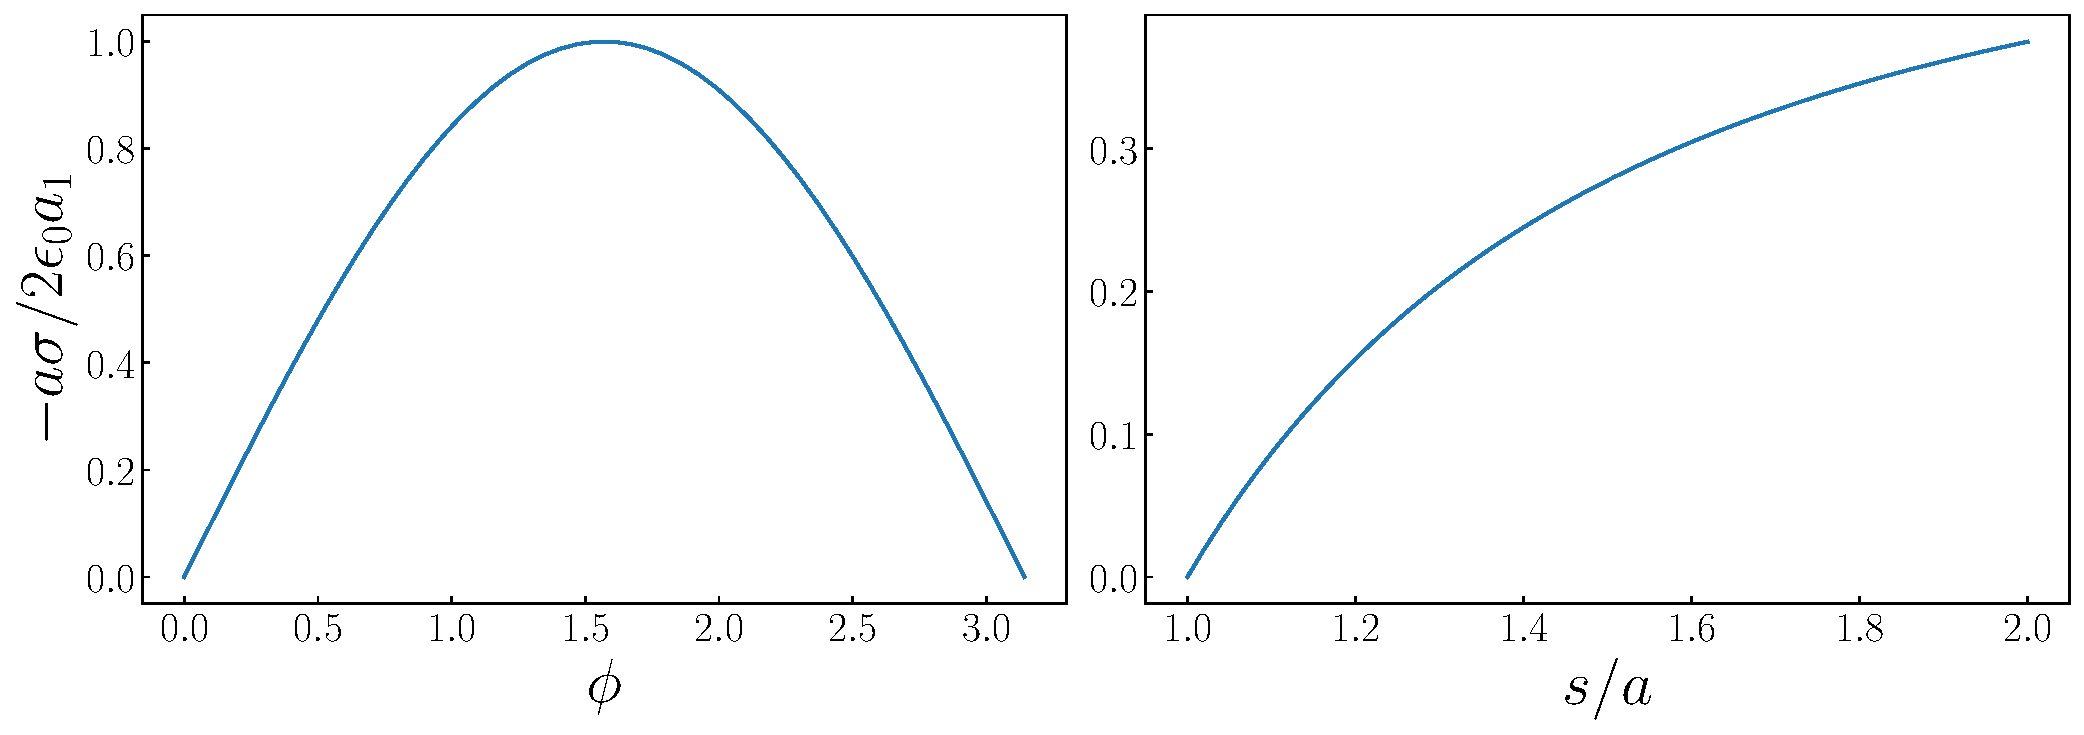
\includegraphics[width=0.7\textwidth]{prob4c.pdf}
   \caption{\textbf{Left}: Plot of surface charge density on the half-cylinder. \textbf{Right}: Plot of surface charge density on the planes. Note that $\sigma(s,0) = \sigma(s,\pi)$, so we could reflect about the $y$-axis and obtain the surface charge density to the left of the half-cylinder as well.}
   \label{}
\end{figure}

The charge on the half-cylinder is
\begin{eqnarray}
    Q = \int_{0}^{\pi} \sigma(a,\phi) a \dd{\phi} = -4 \epsilon_0 a_1
.\end{eqnarray}
Notice that if the cylinder were replaced with a strip of length $2a$, then the total charge would be $2a\epsilon_0(-a_1/a) = -2 \epsilon_0 a_1 = Q/2$.

Clearly this extra charge has to come from the planes surrounding the half-cylinder.
Let us compute the total charge on a strip $2L$, where $L \gg a$:
\begin{eqnarray}
    Q_{L} = 2\int_{a}^{L} -a_1 \frac{\epsilon_0}{a} [1 - (a/s)^2] \dd{s} + Q = \frac{-2\epsilon_0 a_1}{a}\frac{(a - L)^2}{L} - 4 \epsilon_0 a_1 \approx -2 \epsilon_0 a_1 \frac{L}{a}
,\end{eqnarray}
which is just the total charge on a strip of length $2L$ without the cylinder: $2L\epsilon_0 (-a_1/a)$.
Therefore, we have shown that the extra charge $Q/2$ is drawn from the surrounding regions nearby.

}




\end{document}
